In this chapter, we will explore the dual bound quantitative reachability games where one bound is weak. Recall the notion of weak bound: a bound(w.l.o.g say, lower bound) $l$ is weak means, if the weight hits $l$, it never goes below $l$, it stays at $l$ until it goes higher. Also recall that, the weight of a path $\gamma$ with weak lower bound l is denoted as $w\mathord{\downarrow}_{l}(\gamma)$. Here we will consider the case where the upper bound is strong and the lower bound is weak. Note that, the other case can be obtained just by reversing the sign of the weights. Also, we will take the lower weak bound as $0$. Note that, the game with the lower weak bound as $c$ can be simulated with the game with lower weak bound as $0$ converting all weights $w$ to $w-c$. Now, like the strong bound case, we will consider both the one player version and two player version of this game:\\

\section{One Player QR Games with Weak Dual Bounds}

We consider the one player version of this game, where $Q_2= \phi$. We will prove the following theorem:\\

\begin{theorem}
\label{one-player-weak-thm}
Given a game graph $G$ , a strong upper bound $U$ and a lower weak bound $0$, deciding if $P_1$ can win the one player QR games with weak dual bound game in $G$ is is $P$.
\end{theorem}

\begin{proof}
  Before proving it formally, let us look at some intuition: consider a winning strategy $\sigma$ of $P_1$. Intuitively, any outcome of $\sigma$ will not have any positive cycle, as $P_1$ can just ignore the cycle and still win. Hence, it will be either an acyclic path maintaining the objective, or he has to choose a negative cycle where he can rotate enough number of times maintaining the objective, lowers the energy to a certain stable value and then continues forward along the path.\\
  \vskip 0.2cm
  Now, we examine a negative cycle in a graph from a vertex $v$. Starting, from initial energy $0$ from $v$, we will reach $v_1$ in the cycle, where the energy is the highest, let's say $a$. Then, the energy level decreases along the cycle and reaches $v_2$, where the energy level is minimum in the cycle,let's say $x$. Then, it goes back to $v$, with energy, say $y$. Let $b=y-x$. Now, if player $1$ can reach vertex $v$, with at most $U-a$ energy, he will be able to rotate through this negative cycle many times and as the lower weak bound is $0$, after sufficient number of rotation, he can reach $v_2$ with energy level $0$ and reach $v$ with $b$ amount of energy. Hence, we associate the pair $(a,b)$ with the vertex $v$ i.e. if $P_1$ can manage to reach $v$ with at most $U-a$ energy, he can lower his energy level up to $b$ in $v$. The phenomena has been depicted with an example in Figure \ref{energy-negativecycle}.\\
  
  \begin{figure}[htb]
  \label{energy-negativecycle}
  
\begin {tikzpicture}[-latex ,auto ,node distance =1 cm,
state/.style ={ circle,draw,minimum width =1 cm}]

\node[state] (A) [] {$s_1$};
\node[state] (B) [above right=of A] {$s_2$};
\node[state] (C) [right=of B] {$s_3$};
\node[state] (D) [below right=of C] {$s_4$};
\node[state] (E) [ below left=of D] {$s_5$};
\node[state] (F) [left=of E] {$s_6$};
\node (01) [left =of A] {$$};

\path (01) edge [dashed] node[above =0.15 cm] {$10$} (A);
\path (A) edge [bend left =25] node[above =0.15 cm] {$4$} (B);
\path (B) edge [bend left =25] node[above =0.15 cm] {$-2$} (C);
\path (C) edge [bend left =25] node[above =0.15 cm] {$3$} (D);
\path (D) edge [bend left =25] node[below =0.15 cm] {$-2$} (E);
\path (E) edge [bend left =25] node[below =0.15 cm] {$-5$} (F);
\path (F) edge [bend left =25] node[below =0.15 cm] {$1$} (A);
\end{tikzpicture}
\hskip 2cm 
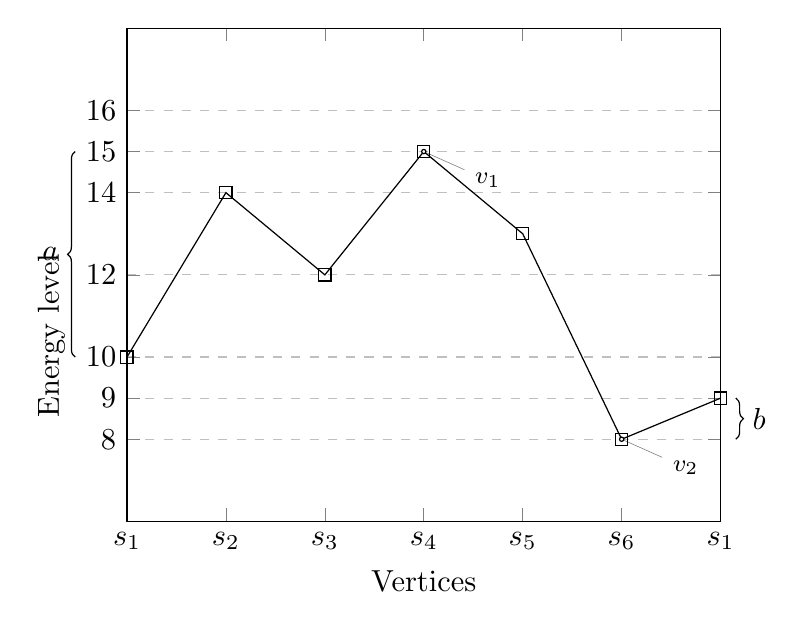
\begin{tikzpicture}[scale=1.1]
\begin{axis}[
    title={},
    xlabel={Vertices},
    ylabel style= {xshift=-20pt},
    ylabel={Energy level},
    clip=false,
    xmin=1, xmax=7,
    ymin=6, ymax=18,
    xtick={1,2,3,4,5,6,7},
    ytick={8,9,10,12,14,15,16},
    xticklabels={$s_1$,$s_2$,$s_3$,$s_4$,$s_5$,$s_6$,$s_1$},
     legend pos=north east,
    ymajorgrids=true,
    grid style=dashed,
]

\addplot[
    color=black,
    mark=square,
    ]
    coordinates {
    (1,10)(2,14)(3,12)(4,15)(5,13)(6,8)(7,9)
    }; 

\node[inner sep=0.5pt,circle,draw,fill=white,pin=-15:\footnotesize $v_1$] 
	  at (axis cs:4,15) {};
	  \node[inner sep=0.5pt,circle,draw,fill=white,pin=-15:\footnotesize $v_2$] 
	  at (axis cs:6,8) {};


\draw[decorate,decoration={brace}]
  ([xshift=-17pt]axis cs:1,10) --
    node[left=2pt] {$a$} 
  ([xshift=-17pt]axis cs:1,15);

\draw[decorate,decoration={brace,mirror}]
  ([xshift=5pt]axis cs:7,8) --
    node[right=2pt] {$b$} 
  ([xshift=5pt]axis cs:7,9);
\end{axis}
\end{tikzpicture}
\caption{Energy level of a negative cycle}

  \end{figure}
  \vskip 0.1cm
  In the example, $U=15$. Hence, $a=5$ and $b=1$, i.e. if player $1$ can reach $s1$ with at most 10 energy level, he can rotate the cycle as much as he wants, and can get the energy level down to energy 1.\\
  Consider a winning path $\rho$ in $G$. Suppose a negative cycle $C$ exists in that path. That means, the path visits the vertex $v_1$, the point with the highest energy level in $C$ at least once. As, the path is winning, it visits $v_1$ with energy level $\leq U$. Hence, if we can compute $(U,b)$ for that vertex $v_1$, we can say that, after visiting the cycle $C$, $P_1$ can rotate around the cycle and get the energy level down to $b$ at $v_1$. Using the idea, we can do the following:\\
  \begin{itemize}
  \item For every vertex $v$, we will check, if it is the highest point of any negative cycle i.e. will check if pair $(U,b)$ exists for some $b \in \mathbb{N} \cup \{0\}$. If yes, then we will calculate the optimal $b$.
  \item We will fill the table $H_{vertex \times steps}$ such that, $H(v,i)=$ The minimum energy level we can have at $v$ after at least $i$ - steps starting from $q_0$. 
  \end{itemize}
  \vskip 0.1cm
  Notice that, if $(U,b)$ pair exists for a vertex $v$, there must exist a negative edge out of it. From the above observation about the energy levels of a negative cycle, it is easy to see that, if $(U,b)$ exists for $v$, from $v$, along the negative cycle, there will be a vertex $u$, where the energy level will be minimum, say $x$. Similarly, there must be a positive weight edge out of $t$. Then, starting from $t$, there will be a path back to $v$. Hence, for every vertex $v$, which has at least one negative edge out of it, we will start with energy level $U$, and for every other vertex $t$ with at least one positive weight edge out of it, we will try to find, if there exists a path of at most length $|V|$, such that it reaches $t$ maintaining the strict upper and the weak lower bound, with energy level $x$, and along the path the energy level never goes below $x$. If we can find such vertex $t$, with energy level $x$, similarly we will try to find, starting from $t$ with $x$ energy, do we have a path of length at most $|V|$ back to $v$, maintaining all the bounds and also such that $x$ is the minimum energy level along the path. Let, we reach $v$ with energy $y$. Then, $b=y-x$. If, we find several such $b$, we will take the minimum one as the optimal. Both the path-checking can be done by simple DFS maintaining the energy level with the vertices. We stop at each path in the DFS when the bound is violated or the length of the path becomes $|V|$. We can also, maintain a counter to remember the minimum energy level seen along the path. Hence, we can compute $(U,b)$ pair for vertices, if exists, in polynomial time.\\
  \vskip 0.1cm
  Once, we have computed the $(U,b)$ pairs for vertices, we can add the following special edges in the graph:\\
  If $(U,b)$ exists for $v$, we add a special loop $v \xrightarrow{\text{:=b}} v$ in the game graph. The idea is, if player $1$ can reach $v$ with at most $U$ energy, he can take some negative cycle in the original graph and get the energy level to $b$ after sufficient many steps. In this new graph, player $1$ can take this special loop and in one step he can lower the energy level of $v$, down to $b$ at one step. Clearly, player $1$ can win in the original graph iff he can win in this new graph with the special transitions.\\
  Now, in this special graph, we will calculate the table $H_{vertex \times steps}$. For any vertex $v$, let \\$e_i=min\{H(u,i-1) + w(u,v) | (u,v)\in E\  \&\  H(u,i-1) \leq U\}$. Then,
   $$
   H(v,i)=
   \begin{cases}
    min(e_i,b), \hskip 0.5cm &\text{if $v \xrightarrow{\text{:=b}} v$ exists and
    $H(v,i-1) \leq U$}\\ 
   e_i, \hskip 1cm &\text{otherwise}
 \end{cases}
 $$
 Now, if for some $i$, $H(T,i)\leq U$, player $1$ wins, otherwise, he loses.\\
 \vskip 0.1cm
 Consider a winning path $\rho$ for player $1$. We have already argued that, there is no positive cycle in this path. Now, the claim is, every special loop can appear at most once in $\rho$. This can be easily seen as the following:\\
 Let, same special transition appears twice in the winning path $\rho$ at $i^{th}$ and $j^{th}$ positions.\\
 \begin{figure}[htb]
 \hskip 2cm
  \begin {tikzpicture}[-latex ,auto ,node distance =1 cm,
 state/.style ={ circle,draw, minimum width =1 cm}]

 \node[state] (A) [] {$q_0$};
 \node[state,label=above:{$i$}] (B) [right= 4cm of A] {$v$};
 \node (01) [right =1cm of B] {$$};
 \node[state,label=above:{$j$}] (C) [right=2.5cmof B] {$v$};
 \node (02) [right =1cm of C] {$$};
 \node[state] (D) [right=4cm of C] {$T$};

 \path (A) edge [dashed] node[above =0.15 cm] {$$} (B);
 \path (B) edge [] node[above =0.15 cm] {$:=b$} (01);
 \path (C) edge [] node[above =0.15 cm] {$:=b$} (02);
 \path (01) edge [dashed] node[above =0.15 cm] {$$} (C);
 \path (02) edge [dashed] node[above =0.15 cm] {$$} (D);
 \end{tikzpicture}
 
 \end{figure}
 \vskip 0.1cm
 Then, the configuration of the path $\rho$ in both the positions are same. Hence, player $1$ can just forget the middle part between the positions, and continue similarly from the $i^{th}$ position, as progressed from the $j^{th}$ position. As, the original path is winning, the new truncated path will also be winning for player $1$.\\
 Now, to prove the correctness of the algorithm proposed earlier, it is enough to prove the following lemma:\\
 \vskip 0.1cm
 \begin{lemma}
 \label{poly-lemma}
  If there exists a winning path for player $1$ in $G$, there exists a winning path of length at most $|Q|^2$ for player $1$.
  \end{lemma}
  \vskip 0.1cm
  \textit{Proof of Lemma \ref{poly-lemma}} Let the optimal shortest winning path for player $1$ has length $>|V|^2$. By pigeon hole principle, $\exists u \in Q$, which appears in the path $|Q|+1$ times. Therefore the path has admitted at least $|Q|+1$ cycles through $u$. As, there can not be any positive cycle in the optimal winning path, all of them are negative cycles. For every negative cycles, the will admit a special transition of the form $v \xrightarrow{\text{:=b}} v$ as shown earlier. Hence, there exists at least $|Q|+1$ special transitions in the path. But the number of unique special transitions are bounded by $|Q|$ and we know, each special transition can appear at most once in the optimal path. Then the contradiction arises\\
 \vskip 0.3cm
  From Lemma \ref{poly-lemma}, it is evident that, calculating $H_{vertex \times steps}$ up to at most $|Q|^2$ many steps are enough.\\
  This completes the proof for our theorem.
 \end{proof}
 \vskip 0.1cm
 Now, we will move to the case for the two player version.
 
 
\section{Two Player QR Games with Weak Dual Bounds}

Now, $Q_2 \not = \phi$ anymore. We will first prove the following lemma about the memory requirements for both the players in the game.\\
\begin{lemma}
\label{mem-lemma}
For two player QR games with weak dual bounds, exponential memory may be necessary for player $1$. For player $2$, memoryless strategies are sufficient.
\end{lemma}
\begin{proof}
As reachability is one of the objective, trivially finite memories are sufficient for both the players. Now, we will show, a class of game graphs, where exponential memory may be necessary for player $1$.\\
\begin{figure}[htb]
\hskip 6cm
\label{expmem-p1}
\begin {tikzpicture}[-latex ,auto ,node distance =1 cm,
state/.style ={ circle, draw, minimum width =1 cm}]

\node[state] (A) [] {$q_0$};
\node[state] (B) [right=of A] {$v$};
\node[state] (C) [right=of B] {$T$};

\path (A) edge [] node[above =0.15 cm] {$U$} (B);
\path (B) edge [loop above] node[above =0.15 cm] {$-1$} (B);
\path (B) edge [] node[above =0.15 cm] {$U$} (C);
\end{tikzpicture}
\caption{Exponential memory is necessary for player $1$ }
\end{figure}

In the game graph of Figure \ref{expmem-p1}, all the vertices are player $1$  vertices and $U$ is the strict upper bound. It is easy to see, player $1$ needs at least $U$- memory to win this game. Considering binary encoding. the value of $U$ is exponential in the size of the input.\\
Now, we will prove that, memoryless strategies are enough for player $2$. Let's fix a winning strategy $lambda$ for player $2$  WLOG, every player $2$ vertices have two outgoing ages. Fix one player $2$ vertex, say $q_2$. Let the weight of the two outgoing edges from $q_2$ are $e_l$ and $e_r$ to $q_l$ and $q_r$ respectively. Now, if any path reaches $q_l$ with at most $w_l$ energy, player $1$ can win from $q_l$ and similarly if any path reaches $q_r$ with at most $w_r$ energy, player $1$ can win from $q_r$. Clearly, if any path reaches $q_2$ with at most $min(w_l-e_l, w_r-e_r)= w^{\prime}$,say, energy, no matter what player $2$ chooses from $q_2$, player $1$ wins. As, $\lambda$ is winning for player $2$, no outcome of $\lambda$ reaches $q_2$ with $\leq w^{\prime}$ energy. W.L.O.G., let $w^{\prime}= w_l -e_l$. It is easy to see that, we can construct a memoryless strategy $\lambda^{\prime}$ for player $2$, such that $\lambda^{\prime}(q_2)=q_l$. Hence, memoryless strategy is enough for player $2$.
\end{proof}
\vskip 0.2cm

Now, based on the previous lemma we can conclude the following theorem:\\
\begin{theorem}
\label{two-player-weak-thm}
Given a game graph $G$ , a strong upper bound $U$ and a lower weak bound $0$, deciding if $P_1$ can win the 2 player QR games with weak dual bound game in $G$ is in $coNP$.
\end{theorem}
\begin{proof}
A priori, lemma \ref{mem-lemma} says if $P_2$ has a winning strategy, he has a memoryless one. Now, we can guess a strategy for Player $2$ (i.e. select one transition per state in $Q_2$) and verify that this strategy is winning for Player $2$ by solving the one player game, which has been proved to be in polynomial time in theorem \ref{one-player-weak-thm}.
\end{proof}
\vskip 0.5cm
\section{A step towards NP}
Now, we prove the existence of a small certificate for the strategy of player $1$. We have already shown that in the original game, player $1$ might need exponential memory. Now, we construct the exponential size graph $G^{\prime}$ with vertices $\langle q_i, E_i \rangle$ explicitly keeping track of the energy level. There is a edge between $\langle q_i, E_i \rangle$ to $\langle q_j, E_j \rangle$ iff there is an edge from $q_i$ to $q_j$ with weight $E_j -E_i$ in the graph $G$, where $E_i, E_j \leq U$. We also add a dead state $q_{dead}$, where any time the energy level goes beyond the upper bound $U$, we move to a dead state. Now, in this exponential graph $G^{\prime}$, the objective of player $1$ is to reach $\langle T,E \rangle$ for some $E \leq U$ from $\langle q_0,0 \rangle$.\\
Clearly, player $1$ has a memoryless strategy to win in $G^{\prime}$ iff he has a strategy to win in $G$. Primarily the idea is that, if player $1$ reaches a same state with same energy level in different paths, all the time he can play the same edge which is the "best" for him and that implies, if player $1$ can win in $G^{\prime}$, he can win memorylessly. Now, we will prove the following lemma:
\begin{lemma}
\label{NP-cert}
For a vertex $q$ in $G$, if there exists $E$ and $E^{\prime} \in \mathbb{N}$ such that, in $G^{\prime}$ player $1$ has a memoryless winning strategy $\lambda$ from $\langle q, E \rangle$ and $\lambda^{\prime}$ from $\langle q, E^{\prime} \rangle$ where, $\lambda(\langle q, E \rangle) = \lambda^{\prime}(\langle q, E^{\prime} \rangle)$, then for every $\langle q,E^{\prime \prime} \rangle$ where $E \leq E^{\prime \prime} \leq E^{\prime}$, there exists a memoryless winning strategy $\lambda^{\prime \prime}$ for player $1$ such that,  $\langle q, E^{\prime} \rangle$ where, $\lambda(\langle q, E \rangle) = \lambda^{\prime \prime}(\langle q,E^{\prime \prime})=\lambda^{\prime}(\langle q, E^{\prime} \rangle)$.
\end{lemma}
\vskip 0.1cm
\begin{proof}
The lemma says simply that, if player $1$ can play same action $a$ from a vertex $q$ with energy level $E$ and $E^{\prime}$, then he can play the same action from $q$ with any energy level between $E$ and $E^{\prime}$. First thing to notice that, it may look like if player $1$ plays a memoryless winning strategy with action $b$ from some vertex $v$ with energy level $E$, then he can play $b$ from $v$ with any energy level $\leq E$ and win. But, this is not true.To see this consider the figure \ref{not_true}. Lets say, $U=4$. So, player $1$ can play self loop action from $\langle v,4 \rangle$ and then win. But, from $\langle v,0 \rangle$ he cannot play the self loop action and win with a memoryless strategy in the exponential graph.\\
\begin{figure}[htb]
\hskip 6cm
\label{not_true}
\begin {tikzpicture}[-latex ,auto ,node distance =1 cm,
state/.style ={ circle, draw, minimum width =1 cm}]

\node[state] (A) [] {$q_0$};
\node[state] (B) [right=of A] {$v$};
\node[state] (C) [right=of B] {$T$};

\path (A) edge [] node[above =0.15 cm] {$4$} (B);
\path (B) edge [loop above] node[above =0.15 cm] {$-1$} (B);
\path (B) edge [] node[above =0.15 cm] {$1$} (C);
\end{tikzpicture}
\caption{Player $1$ cannot play same memoryless strategy from $\langle v,4 \rangle$ and $\langle v,0 \rangle$}
\end{figure}
But from $\langle v,1 \rangle$ he can play the same action and win with a memoryless strategy. So, the lemma says, from $\langle v,3 \rangle$ and $\langle v,2 \rangle$ also, he can play the same self loop action and win with a memoryless strategy in the exponential graph.\\
Now, we will go to the proof of the lemma. 
\fcolorbox{blue}{red}{Trying to work out the proof.}
\end{proof}
\vskip 0.5cm
Now, the previous lemma takes us to a step towards proving that the $2$ player QR game with weak dual bound is in NP. This is because, though the energy levels are exponential when expressed in binary, the number of actions player $1$ can take from each vertex is linear in size. Now, lemma \ref{NP-cert} suggests that, for a fixed vertex we can group energy levels into intervals from where we can take the same action, hence the number of groups in also at most linear in size.\\
This works as our short certificate. Given a game graph $G$ with weak dual bounds objective, we can guess a grouping of energy levels to produce a game graph $G^{\prime \prime}$ with vertices as $\langle s, I\rangle$, where $s$ is a vertex in $G$ and $I$ is an interval of energy levels. Note that, $G^{\prime \prime}$ has at most $O(n^2)$ many vertices. After guessing the short certificate, the verification process will be to check reachability of $\langle T, I\rangle$ for any interval $I$ and target state $T$ from $\langle q_0, I^{\prime} \rangle$, with $I^{\prime}$ containing 0. But, we do not know, how to execute this verification process in polynomial time. 
\section{Conclusion}
In this chapter, we have showed that QR games with weak dual bounds are in $P$ for the single player case and is in $coNP$ for the two player case. We also believe that the two player version of the game is in $NP$. We have shown the short certificate for the problem, but unfortunately could not prove the verification part.\\
This ends all the QR game versions with bounds on weight functions. In the next chapter, we will introduce a new QR game, with a notion of bound on number of violations.